\section{Colonel Blotto}\label{sec:colonel blotto}
For the representation of Colonel Blotto strategies in a genome I simply used
the simple binary genome from part A of the assignment and decided that 5 bits
represented one value, to get that into the desired range I divided the value by
three. This gives a range of 0 to 10, but it does skew the numbers in favour of
10 slightly. In figure \ref{fig:colonel blotto genome} you can see how the
genome is sliced to make one value.

\begin{figure}[h!]
	\centering
	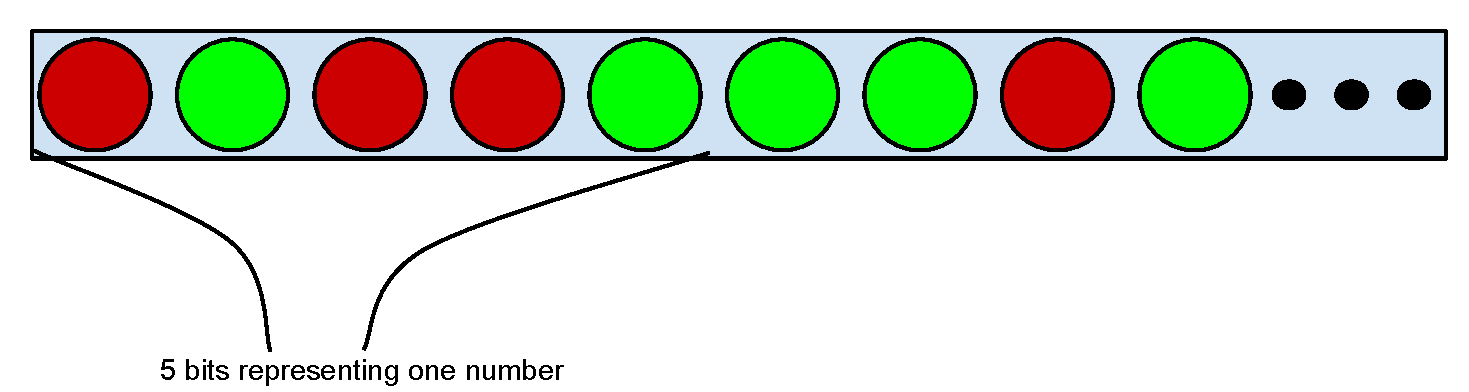
\includegraphics[scale=0.5]{blotto-genome.pdf}
	\caption{Colonel Blotto genome representation}
	\label{fig:colonel blotto genome}
\end{figure}

To convert the binary genome, which consist of five times the number of battles,
into a phenotype containing a list of numbers I just retrieve the bits
converting five bits at a time into a number and then dividing by three. Then I
sum over all those values and divide each value by the sum thus normalizing
them. I keep both the original and the normalized list of numbers in the colonel
blotto phenotype.

\subsection{Population Entropy}\label{sec:population entropy}
The population entropy is interesting in this problem because it represent the
coevolution of the strategies. Since each strategy competes with all the other
strategies for dominance the best strategies will most likely mate. It will then
be better if new strategies takes the best from the previous population, meaning
the whole population becomes more homogeneous. In other words each strategy
"tries" to approach the best strategy which means that the average entropy will
decrease. This shows off the coevolution taking place through the evolutionary
run.

\subsection{Blotto Settings}\label{sec:blotto settings}
For the runs documented later I tried a few configurations. One problem was that
random seed affects the result more then anything so the settings are just
chosen on the basis of what I think might work and have seen work in a couple of
runs locally.

\begin{tabular}{| l | c | p{7cm}|}
	\hline
	Variable & Value & Description \\
	\hline
	\hline
	Generations & 100 & I chose 100 since this should be more than enough
	for the phenotypes to converge and since the assignment states that 100
	should be more than enough \\
	\hline
	Population size & 30 & I tried with fewer populations and saw a much more
	rapid growth with 30, even though the assignment states 20 I decided to
	use 30 since it had work well before and seemed to be good for this
	problem to \\
	\hline
	Protocol & full\_generational & I used this as it seems to work quite
	well, the way elitism is implemented also affects this and mens that it
	does not stray that much away from generational mixing \\
	\hline
	Mechanism & tournament & Since tournament did so much better than all
	the other selection mechanisms I really only tested with Tournament
	selection \\
	\hline
	--cross\_rate & 0.8 & Even though 1.0 worked well for the One-Max
	problem for this 0.8 seemed better during testing. This can be explained
	by the fact that it in some sense increase the elitism, but with a
	random chance \\
	\hline
	--cover\_rate & 0.5 & For the cover rate I chose to run with 0.5 because
	this seem to work well and smaller cover rates have not done
	particularly well \\
	\hline
	--mutation & 0.01 & As mentioned earlier a small mutation rate seem to
	work well and this also does make some intuitive sense because it means
	that there won't be to many changes which can effect the fitness of an
	individual \\
	\hline
	--elite & 3 & The elitism was again placed at 3 to get a better result
	than with no elitism, since this is affected by the chosen protocol I
	think this makes sense to include some elitism. The number was chosen
	because it seemed that this was the smallest value which had an effect
	\\
	\hline
	--k & 10 & The size of tournaments was chosen on the basis of how large
	the total population size \\
	\hline
	--e & 0.05 & This value was chosen on the basis that we want the best
	individuals further, but we also want some variation my thinking here
	was that this is large enough to include some variation, but small
	enough to mostly favour the best \\
	\hline
	--seed & 26150 & Just a randomly generated seed from \$RANDOM \\
	\hline
\end{tabular}

\subsection{Blotto Results}\label{sec:blotto results}
In table \ref{tab:blotto} we can see the results of all the blotto runs.
Since all of the runs got the same starting point, only the battle parameters
differed between runs, the starting entropy was the same for equal battle sizes,
for 20 it was 3.95 and for 5 it was 1.98. The decision
to have the start with the same population always was to ensure that it is only
the war parameters that differ in order for us to properly see their results.
Note also that the final entropy might not reflect the whole story as the
population can diversify later in the run.

\begin{landscape}
	\begin{table}
		\begin{tabular}{| c | c | c | p{10cm} | c |}
	\hline
	Battles & Redeployment & Loss fraction & Description &
	Entropy(End) \\
	\hline
	\hline
	20 & 0.0 & 0.0 & This run converged quite nicely to one stable strategy,
	which it did after only about 34 generations. & 0.61 \\
	\hline
	20 & 0.0 & 0.5 & Some what of a periodic shifting. & 1.06 \\
	\hline
	20 & 0.0 & 1.0 & Quite random distribution, but there are some
	periodicity in that it shifts between distributing for mostly the start
	or more evenly split among more of the intermittent battles. & 2.52 \\
	\hline
	20 & 0.5 & 0.0 & Quite random, some periodicity late which is lost, but
	   all in all quite random & 2.64 \\
	\hline
	20 & 0.5 & 0.5 & Again quite random, some phenotypes survive a couple of
	   rounds, but the loses to another & 1.81 \\
	\hline
	20 & 0.5 & 1.0 & Some periodicity in that the third is goes from 0.0 to
	 something then back to 0.0 in the last few runs. & 1.40 \\
	\hline
	20 & 1.0 & 0.0 & Mostly random, some survive more than one round and
       some are quite equal, but no major trends. & 2.65 \\
	\hline
	20 & 1.0 & 0.5 & Mostly random again, few surviving and very few
   similarities compared to last run. & 3.16\\
	\hline
	20 & 1.0 & 1.0 & Somewhat periodic in that the general trends reoccur. &
	1.62 \\
	\hline
	5 & 0.0 & 0.0 & Again a very stable strategy, extremely fast convergence
	  & 0.07 \\
	\hline
	5 & 0.0 & 0.5 & Here we see convergence to one strategy for then to
     shift to another strategy which seemed to have converged & 0.50 \\
	\hline
	5 & 0.0 & 1.0 & Same story as the last one, for a long time one strategy
	  seem to be best, for then randomly to shift to another one which is
	  then used further & 0.66 \\
	\hline
	5 & 0.5 & 0.0 & Quite a lot of periodicity some strategies appear then
	disappear then reappear towards the end, seem to switch between two. &
	0.07 \\
	\hline
	5 & 0.5 & 0.5 & Seems quite random, some strategies survive some rounds,
	  but doesn't seem to be much periodicity & 1.58 \\
	\hline
	5 & 0.5 & 1.0 & Seem to stabilize slightly, but again it is only for the
	  last 10 or so generations and within there some randomness occur &
	0.85 \\
	\hline
	5 & 1.0 & 0.0 & Periodic shifting between two strategies, but some
    slight randomness, this seem to be the most periodic of all so far. & 1.49 \\
	\hline
	5 & 1.0 & 0.5 & Some periodic shifts, not as clear as the one above, but
	  there seem to be some. & 0.50 \\
	\hline
	5 & 1.0 & 1.0 & Fairly random with some convergence towards the end &
	0.53 \\
	\hline
\end{tabular}
	\label{tab:blotto}
	\caption{Table showing the results}
\end{table}
\end{landscape}
